%!TEX root = thesis.tex

\chapter{Modelling Pre Evacuation Behavior in Agent Based Simulations Of Crowds}
\label{chapter:PreEvacuationBehavior}

\section{Introduction}
\label{intro}
Ideally, when a fire starts a fire alarm goes off; all occupants hear this alarm and use the nearest safe exit to leave the building. However, this is hardly the norm. In many cases, occupants are desensitized from hearing false alarms and often do not start to evacuate until they are completely sure that it is needed. On January 19, 2000, a fire in Boland Hall in Seton Hall University killed three students because they had ignored the fire alarms assuming they were false~\cite{Berry:2000us}. This uncertainty about the authenticity of the first sign of danger isn't an isolated incident~\cite{Proulx:2003tc,Purser:2001ts,Tong:1985wn}. Hence, when studying the behavior of evacuees, it is necessary to study and understand their actions from the time at which the fire started right up until the point where the last person evacuated~\cite{Tong:1985wn}. Modeling and simulation is one approach for analyzing and understanding egress behavior.

Software that simulates crowd egress is necessarily very complex because crowd egress from a building is itself a very complex system with lots of interacting elements (people, fire, alarms, etc.) each of which can cause different complications in the system. One of the most popular methods for studying and modeling complex systems is through Agent Based Models (ABM). In ABM, a set of heterogeneous, intelligent entities called agents are programmed with behavior approximating humans and placed in a partially observable environment. Asynchronous interactions between agents result in macro-level dynamics which can help observers learn more about the system.

Pre-evacuation uncertainty and investigation are features of human behavior during egress that are rarely considered in models. Pre-evacuation refers to the period of time that elapses after the start of the fire alarm before the person starts evacuating. While some models~\cite{Tsai:2011tz} do have a simplified model of pre-evacuation behavior, they fail to model it in enough detail to enable their extension to more general cases. For example, a fire alarm could have different effects based on the clarity and believability of the alarm~\cite{Kobes:2009jx,Paulsen:1984ti}. This variability is hard to model in existing models of pre-evacuation behavior. Also, during an evacuation people exchange event and environment related information with other evacuees. Evacuees are unlikely to follow blindly any and all messages that they receive. There is a variability in the \emph{trust} in messages received that can have different effects on egress. This is rarely considered in existing models.


In this paper, we present one aspect of a behavioral model for Agent Based Modeling of crowd egress which we call the IBEVAC (Information Based Evacuation) model. This behavioral model models evacuees as information processing entities. More specifically, in this paper we introduce the information-based event identification and communication system that is used in IBEVAC. The evacuees identify and process information in terms of event cues which exist throughout the environment. The importance of modeling pre-evacuation behavior and a communication system is illustrated through experimentation.

\section{Related Work}
\label{LitRev}


A fire evacuation is a complex situation to model and simulate. One large component of this complexity is the need to understand the behavior and decision making of the people taking part in it. There are a lot of conflicting theories on how humans behave in emergencies and why they behave as they do. However, there are also certain parts of human nature that are generally accepted to be true, such as the constant search for information~\cite{Proulx:2003tc,Tong:1985wn,Ozel:2001tn,Sime:1983uy}. This section first summarizes the existing knowledge of human behavior during egress with special emphasis on pre-evacuation behavior. Following this, some existing models of pre-evacuation behavior and communication is presented.

\subsection{Pre-evacuation Behavior}
\label{PreEvacuationBehavior}

Several studies of human behavior during emergency egress~\cite{Kuligowski:2005tt,Ozel:2001tn,Proulx:2007ul}, have shown that an evacuee's first reaction after realizing that there is an unusual situation is to investigate and gather more information about the situation. Evacuation starts only once the need for evacuation is established. \emph{Cues} are the key to understanding this transition from realization to investigation and, eventually, to evacuation. Cues are certain changes in the environment that indicate that something is wrong or different from normal~\cite{Sime:1983uy}. They come in a variety of different forms. Fire and smoke are the typical and most unambiguous cues for an evacuation. Fire alarms and people running about are examples of more ambiguous cues. According to Proulx~\cite{Proulx:2007ul}, an ambiguous cue by itself does not cause a person to initiate investigation. Rather, the cue has to persist for a period of time before investigation begins.

There have been several surveys, interviews and other studies of the factors that influence evacuation and pre-evacuation behavior. Kuligowski~\cite{Kuligowski:2009un} summarized the key findings of these studies and compiled a list of factors that influence pre-evacuation behavior. She suggested that the period that we term as pre-evacuation itself consists of two phases. Phase 1 is called \emph{perception}. This refers to the perception of some unusualness in the current situation. Kuligowski calls the next phase \emph{interpretation}. During this phase, the person searches for more information to verify whether a fire has actually started and if it actually poses a threat that needs to be handled. Several others~\cite{Ozel:2001tn,Proulx:2007ul,Tong:1985wn} have also emphasised the importance of this phase though sometimes under different names. Regardless of what it is called, this phase consists of two parts~(1) defining the situation as a fire and~(2) defining the risk that the situation poses.

% Explaing milling somewhere here.

Kuligowski categorized the factors that influence these phases into two types: occupant based factors and cue based factors. Occupant based factors are intrinsic characteristics of the evacuee like age, experience, gender, etc. One of the factors that encourage the programmatic implementation of cue based factors is the fact that the effect of a cue can be explained to be caused by the nature and characteristics of the cue rather than the specific cue. In other words, each cue can be described in terms of its ambiguity, consistency with other cues and its source and it is this description that determines the effect of the cue.


\subsection{Existing models}
\label{ExistingModels}

As mentioned in Section~\ref{intro}, there are very few existing models that take the pre-evacuation period into consideration. Pires~\cite{Pires:2005gs}  modeled the pre-evacuation decision making of an individual using a simple Bayesian Belief Network~(BBN). Fran{\c c}a et al.~\cite{Franca:2009wq} created a simulation model of the development of panic behavior during emergency egress. This model implemented the hysterical belief theory~\cite{Torres:2010tj} and modeled how panic first develops and then evacuation happens. It also had a basic communication system through which agents exchanged mood information (which is a key factor in the development of panic) by using the grid based environment as a medium for communicating messages. Despite pre-evacuation behavior being modeled in some detail, it is not possible to extend this model to replicate the heterogeneity in people's reaction to cues. ESCAPES~\cite{Tsai:2011tz} is a fairly recent model that takes into account some factors like the spread of knowledge, fear and emotion between the different evacuees. These factors are used to create a simplistic model of pre-evacuation behavior. The event identification and communication model proposed in this paper have been influenced by these models but is unique in the way that the diversity of cues and their effects can be considered.

% \section{The IBEVAC Model}
% \label{IBEVAC}


% \begin{figure}[!tb]
% \centering
% 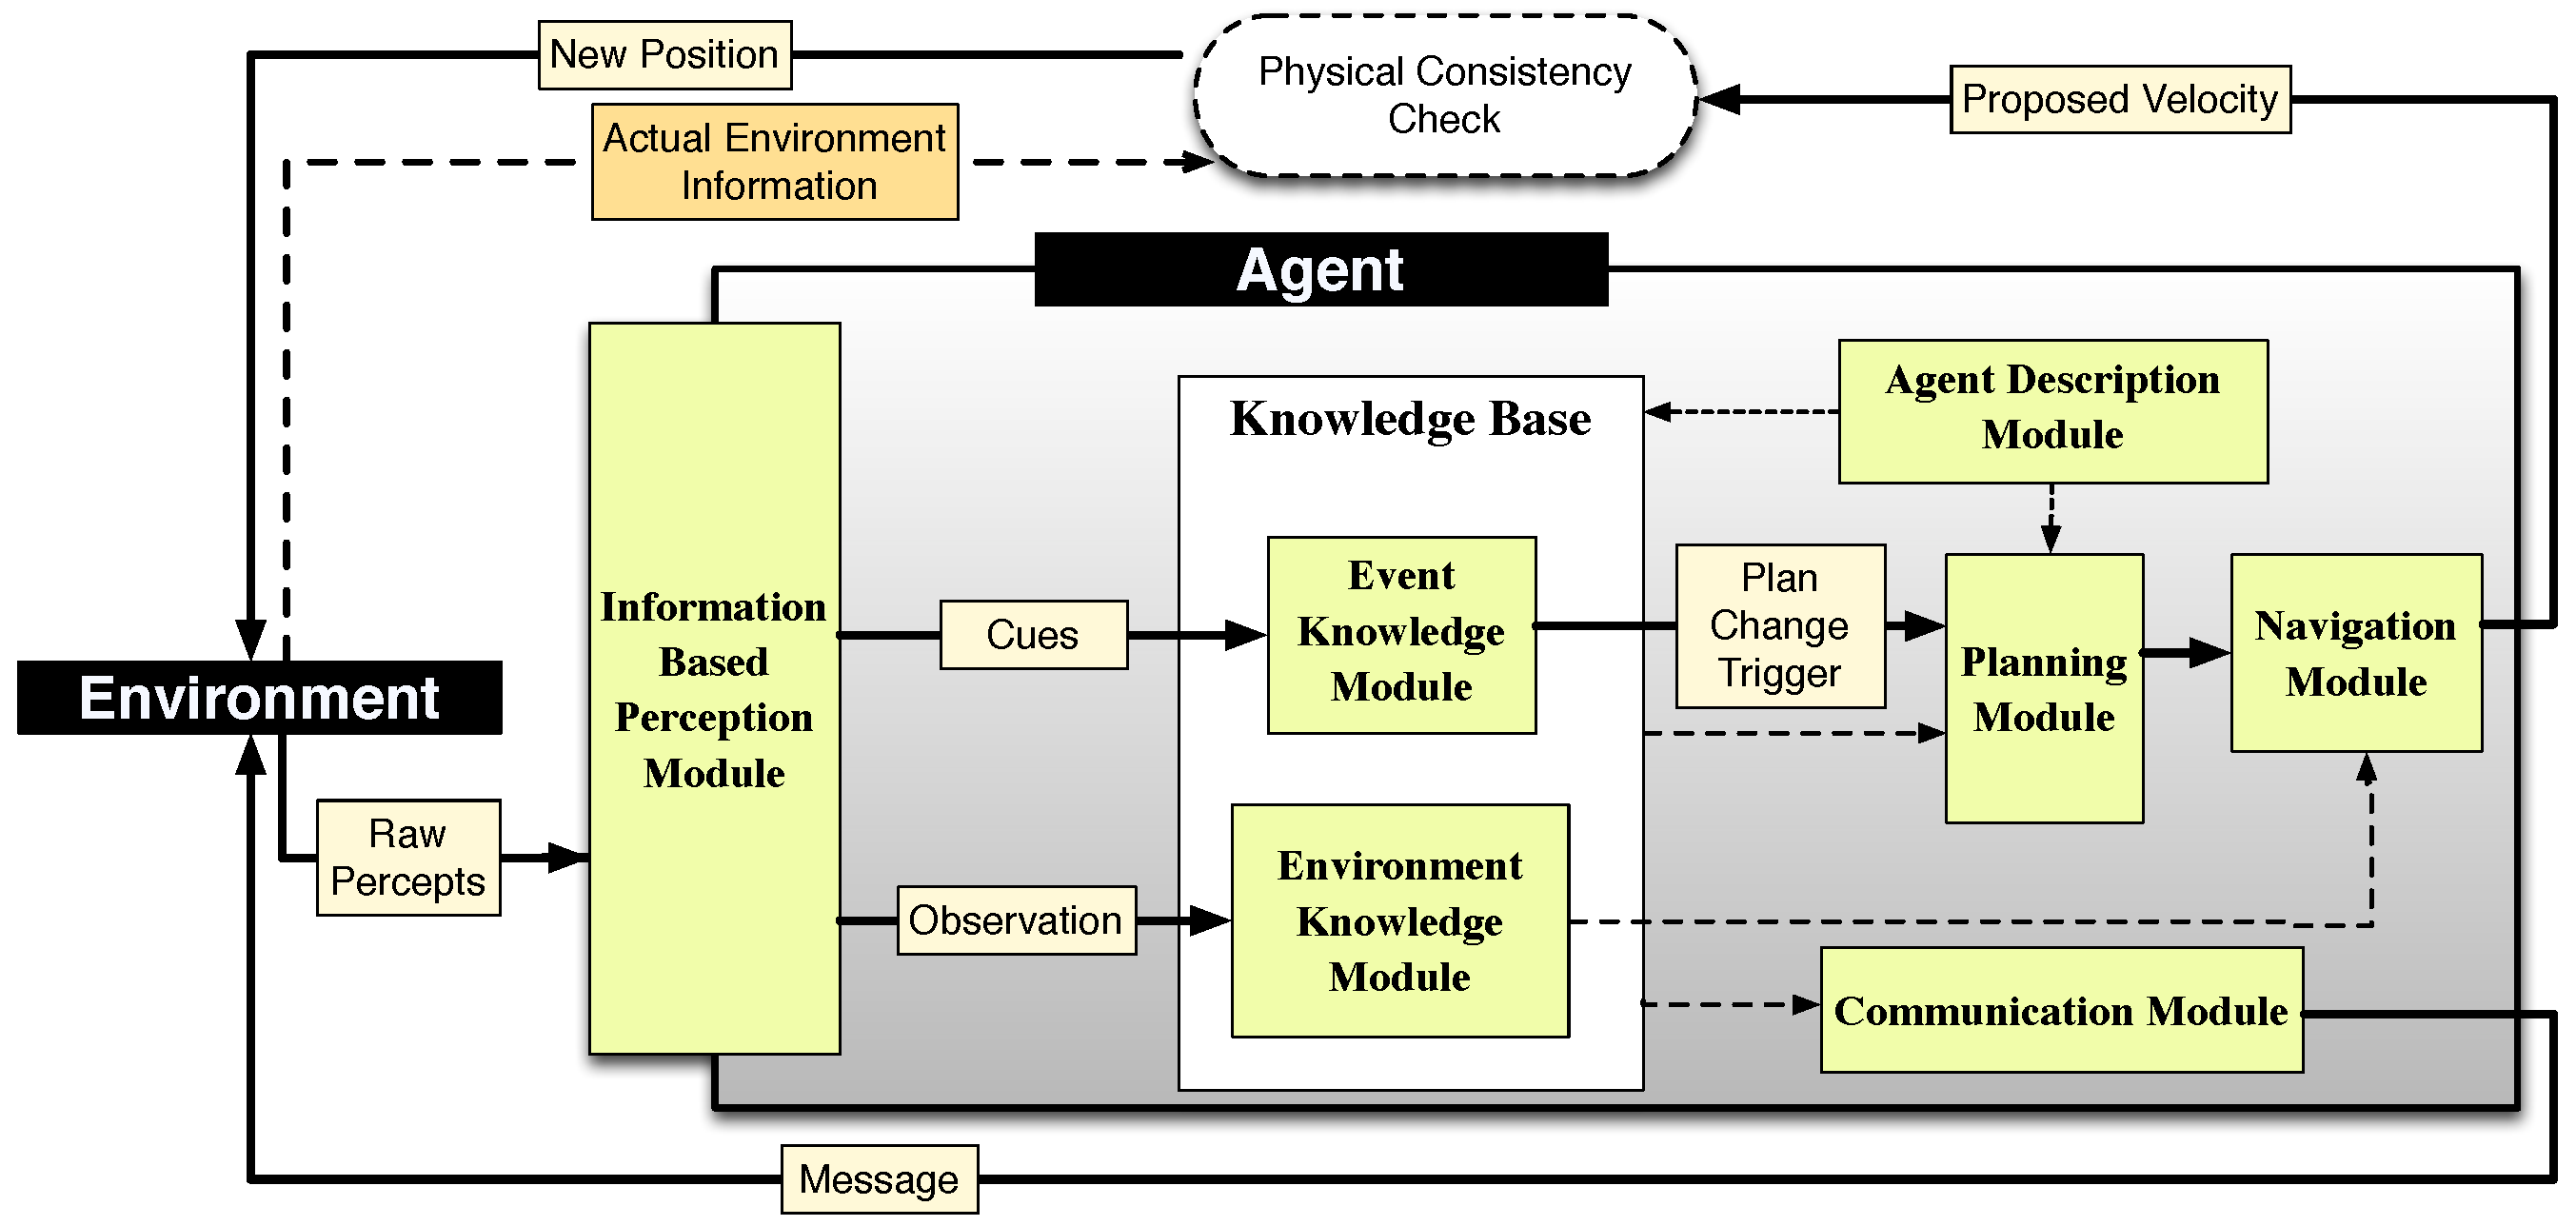
\includegraphics[height=1.9in]{SimplifiedAgentArchitecture}
% \caption[The Agent Architecture]{An illustrated representation of the IBEVAC agent architecture}
% \label{fig:AgentArchitecture}
% \end{figure}

% This section gives an overview of the modular IBEVAC agent architecture. Figure~\ref{fig:AgentArchitecture} shows this architecture. There are many objects or actions that an agent can sense or observe in the environment. We call these \emph{raw percepts}. According to their sources, they can be classified as \emph{observations} from the environment and \emph{messages} from other agents. The Information Based Perception~(IBP) Module is the only gateway through which the agent receives information from the environment. This module is explained in more detail in~\cite{Viswanathan:ut}. The IBP Module passes a percept to the Knowledge Base.

% The \emph{Environment Knowledge Module} stores a representation of the layout of the environment that is formed as a result of the observations of the agent. Information regarding accessibility of links is also stored. As a detailed discussion of this module is beyond the scope of this paper, all agents are assumed to have complete knowledge of the layout. However, agents can learn about inaccessible links only through direct observation or through messages from other agents. The {\em Event Knowledge Module} is the focus of research in this paper. It stores the agent's beliefs about the current state of the environment. Cue perception alters these beliefs and triggers a state change in the agent which is then handled by the Planning Module. This Module is explained in more detail in section~\ref{EventIdentification}.

% The intrinsic characteristics of the agent like the agent's size, speed, mass and social role are stored in the {\em Agent Description Module (ADM)}. It is also responsible for determining the strategies and actions taken by the Planning Module and in determining the effects of the cues on the Event Knowledge Module (Section~\ref{EventIdentification}). The {\em Planning Module} stores the current state of the agent i.e. whether it is exploring, milling or escaping and creates a plan of action for the agent as a set of goals. Each goal is a location that is passed to the Navigation Module.

For the purpose of this paper, three kinds of behavior are modeled: normal behavior where the goal is the center of the \emph{home} room of the agent, for milling behavior the agent gathers with other agents at the nearest \emph{corridor} (See Figure~\ref{fig:layout}) and during escape the agent heads towards the nearest exit.

Communication between agents is facilitated by the {\em Communication Module}. It transmits messages to agents within a communication range. The working of this communication is explained in more detail in Section~\ref{EventIdentification}. The {\em Navigation Module} uses a four level navigation system. At the highest level, a logical path is determined in terms of rooms to be crossed from the agents current location to the goal. From this logical path, spatial way points or locations are extracted by the next level. The third level determines a possible collision free path to the farthest visible spatial way point. Finally, a physics engine ensures that objects don't pass through other objects.

\section{Event Identification and Pre-evacuation Behavior}
\label{EventIdentification}

% First explain how cues are modeled
It is known that the ambiguity, source and consistency of the cue~\cite{Kuligowski:2005tt,Sime:1983uy,Tong:1985wn} are the key factors (Section~\ref{PreEvacuationBehavior}) in determining the effect of a cue. In the IBEVAC model, this is used in modeling all cues in the same way. Each object or event that is to be perceived as a cue implements a \emph{Cue interface} which ensures that each cue can be explained in terms of its ambiguity, source and consistency. This is one of the key novelties of IBEVAC's approach to behavior modeling. Each cue is located at a particular location in the environment and is sensed by agents when within their perception range.

% Next explain how these cues affect the event knowledge module and the idea of buckets and thresholds. One line about how these thresholds are connected to different stages.
Once perceived, these cues are passed to the Event Knowledge Module. The  module has a \emph{bucket} of information corresponding to \emph{uncertainty} and another corresponding to \emph{fire}. When a cue is perceived, appropriate amount of information is added to the appropriate bucket(s) based on the ambiguity level. A less ambiguous cue contributes more information. For each bucket, a \emph{threshold} is initially fixed by the ADM. When the amount of information in a bucket overflows the threshold, a trigger is sent to the Planning Module to change the agent's state and strategy.

% Following this explain how messages contain message cues and additional information.
Communication is implemented as \emph{messages} sent from one agent to the other. Each message has a message cue and environment information. The message cue works just as other cues. Here the term ambiguity is used to refer to the trustworthiness of the source of the information. In this paper, the environment information that is passed is only about the inaccessible paths in the map. % Finally summarize what all happens during a simulation.
During an IBEVAC simulation, a cellular automata based fire model and a simple finite difference smoke model are executed. This creates fire and smoke cues at locations near the fire. As soon as the fire starts, fire alarm cues are placed all over the environment. Agents react to these cues and mark observable pathways that are blocked as inaccessible in their Environment Knowledge Module. All agents either escape or are killed at the end of the simulation.



\section{Results}
\label{Results}

% Outline what are the things that we expect to demonstrate
Experiments were conducted using IBEVAC to demonstrate the effect that cue perception and communication can have on egress. Both experiments were conducted on the two floor office environment shown in Figure~\ref{fig:layout}. Simulations were conducted with 200 agents randomly distributed all over the environment and data was collected after averaging over 100 replications of the simulation.

\begin{figure}[!tb]
\centering
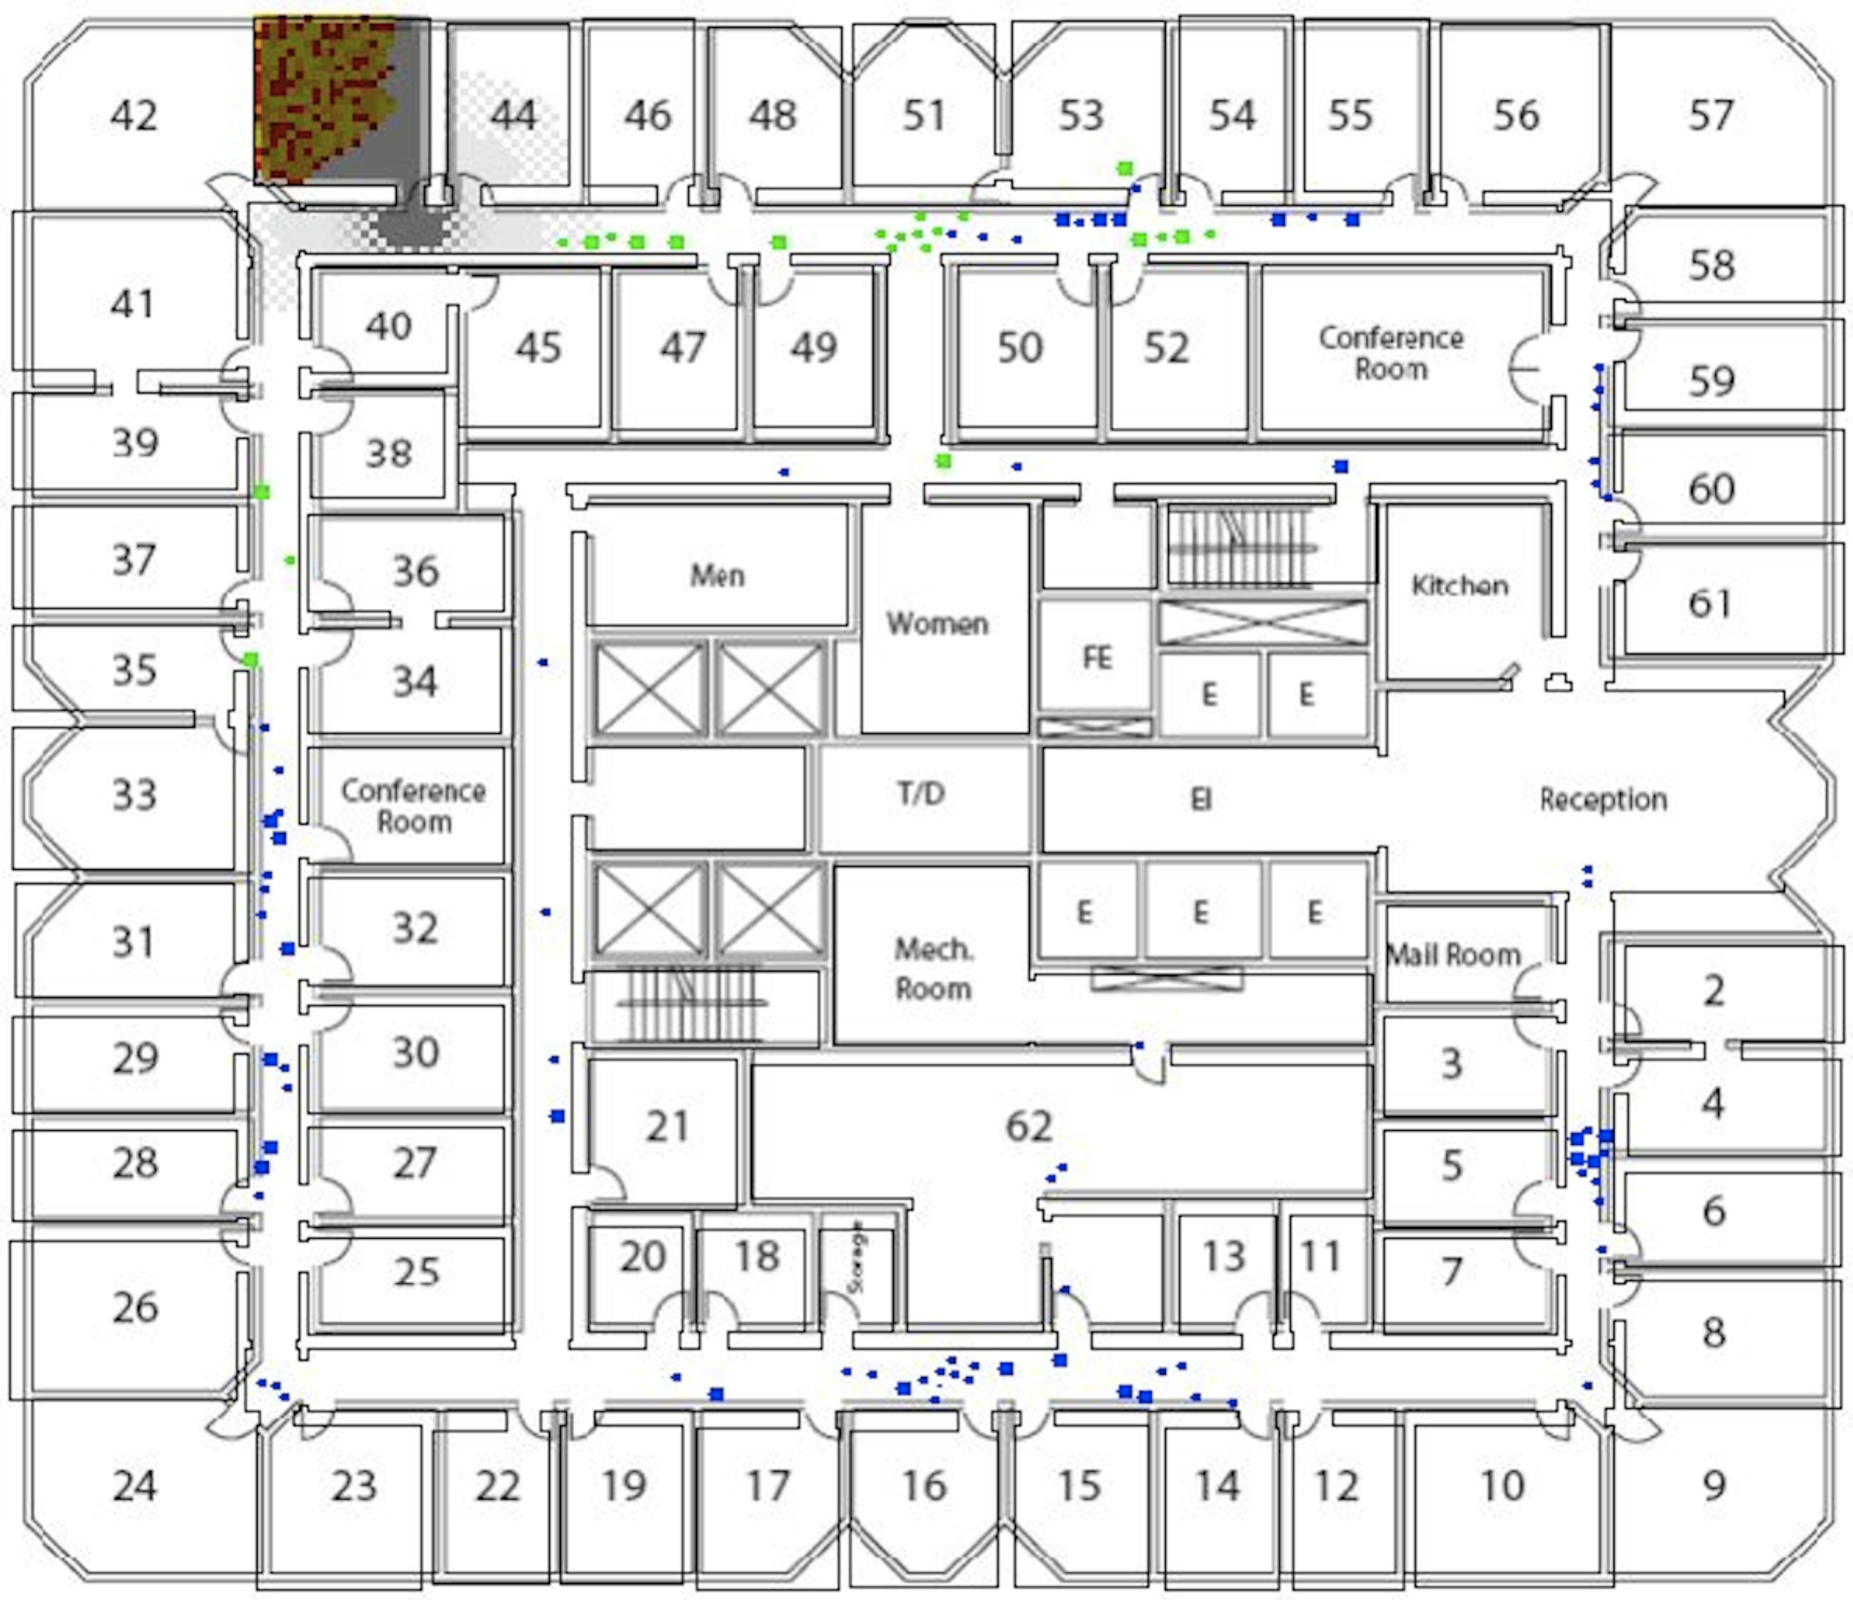
\includegraphics[height= 2.5in]{layout}
\caption[The Environment Layout]{First of two floors from World Trade Center, California. Fire is started in the corner room and generates smoke. Fire kills agents. Smoke depending on concentrations slow or kill agents. The longer rectangles are corridors connecting rooms and the open area on the right center is the exit.}
\label{fig:layout}
% Change to my figure
\end{figure}

% Explain the layout of the environment, the settings and parameters

\subsection{Experiment 1: The effect of fire alarm clarity}
\label{experiment1}

In this experiment, the effect that fire alarm cue clarity and ambiguity has on egress was examined. It is assumed that the fire alarm can be heard clearly at every location on the map; so cues are placed in every room. A fire alarm with a simple ringing sound is much less clear and more ambiguous than a public announcement system that explicitly states that it is not a drill and gives real time updates about the situation. To examine the effect of this difference in clarity, the experiment was repeated for different values of ambiguity (from 0.0 - 1.0). The blue curves in Figure~\ref{Graph1} show the error plot of the survival percentage and the one in Figure~\ref{Graph2} the average time taken for last agent to start evacuating for this experiment. As expected there is a significant drop in number of survivors as the ambiguity of the alarm increases. Also, the later an agent starts evacuating, the lesser is his chance for survival.



% Think about someway to plot the distribution of evacuation start time against ambiguity. This might be a better measure.

\subsection{Experiment 2:  The importance of communication}
\label{experiment2}

In this experiment, the effect of message trustworthiness (ambiguity) is modeled. The fire alarm ambiguity is kept at 1.0 to minimize its interference with the effect of message cues. Similar to experiment 1 the cue ambiguity is varied from 0.0 to 1.0. The green curves in Figure~\ref{Graph1} and Figure~\ref{Graph2} show the results for this experiment. However, both these data are collected for agents in the lower floor only. This is because none of the agents on the higher floor start evacuating as they neither observe the fire nor get a message from other agents about the fire. A similar trend can be observed where the survival rate decreases with increasing ambiguity. The green curve in Figure~\ref{Graph2} flattens out towards the end because in both these cases, the agent's trust in other agents is so less that the only reason they start evacuating is because of the smoke or fire itself. Another thing to note is that even if all agents are completely trusted (ambiguity=0), the last agent still takes a long time to start evacuating because it takes a long time for the information to propagate to it. This can also explain why there is such a dramatic change in the effect of slight change in ambiguity of the fire alarm cue as opposed to a change in ambiguity of the message cue.


%Might it have made more sense to carry this experiment out slighlty differently from the other one in varying the number of high trust and low trust ppl? rather than one unique ambiguity value for all messages?

% \begin{figure}[!tb]
%    \centering
% 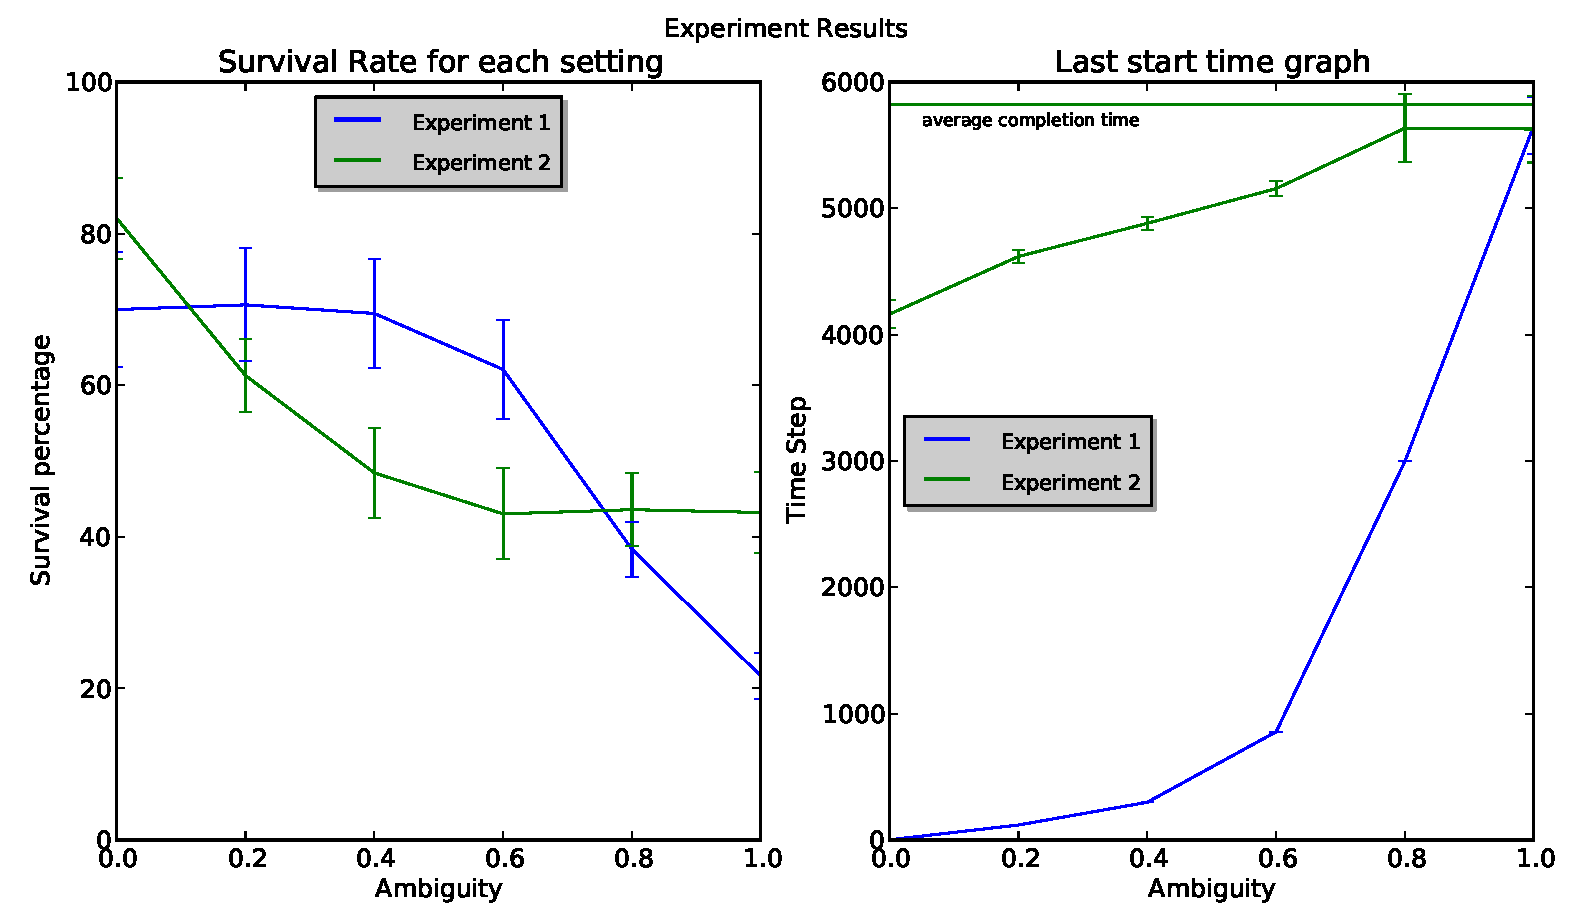
\includegraphics[width=\textwidth]{results}
%   \caption{Observations from 100 replications of each setting of the IBEVAC Simulation}
%   \label{Exp}
%  % Change graph to have average survival rate instead of average number survived.
% \end{figure}
\begin{figure}[!tb]
   \subfloat[Average Survival Rate]{\label{Graph1}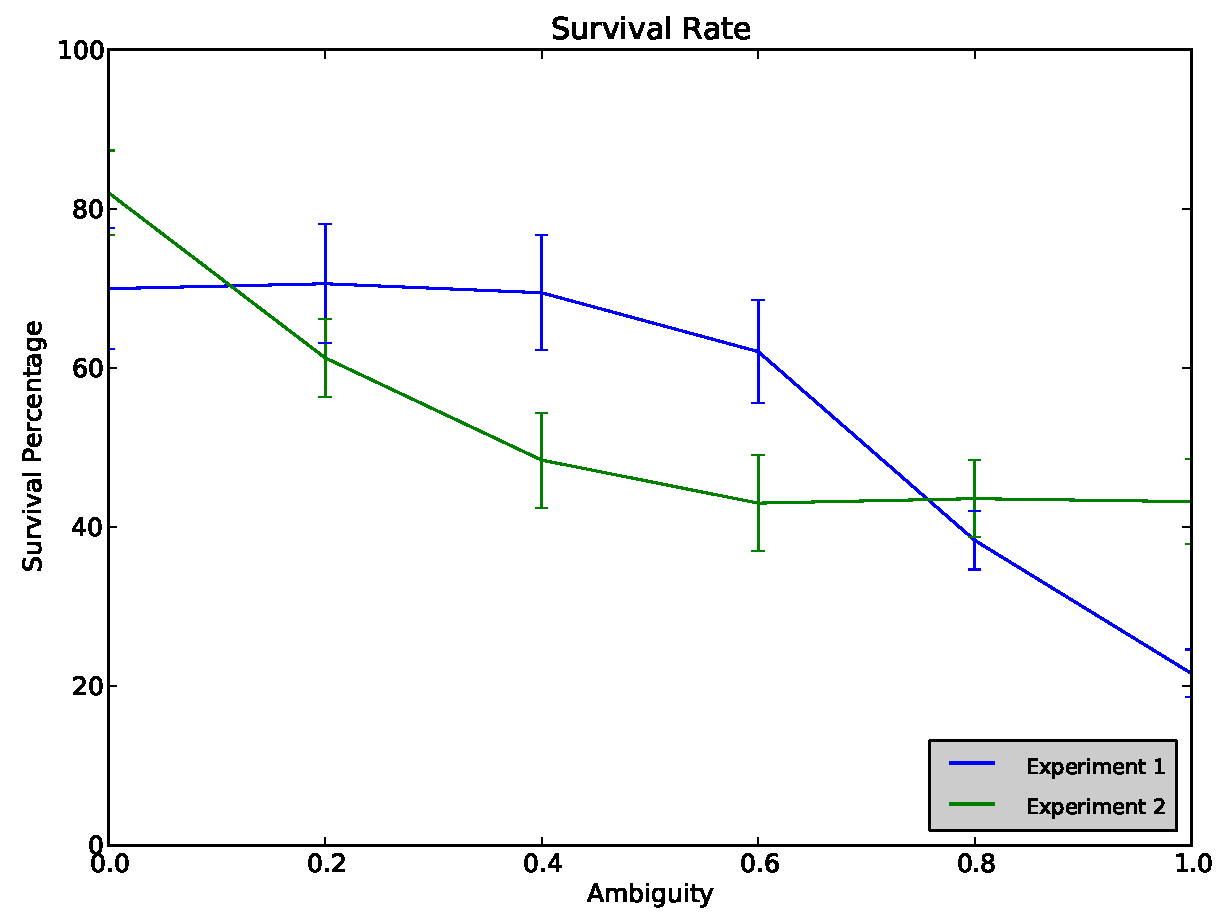
\includegraphics[width=6cm,height=6.2cm]{Exp1}}
   \subfloat[Last Agent Start Time]{\label{Graph2}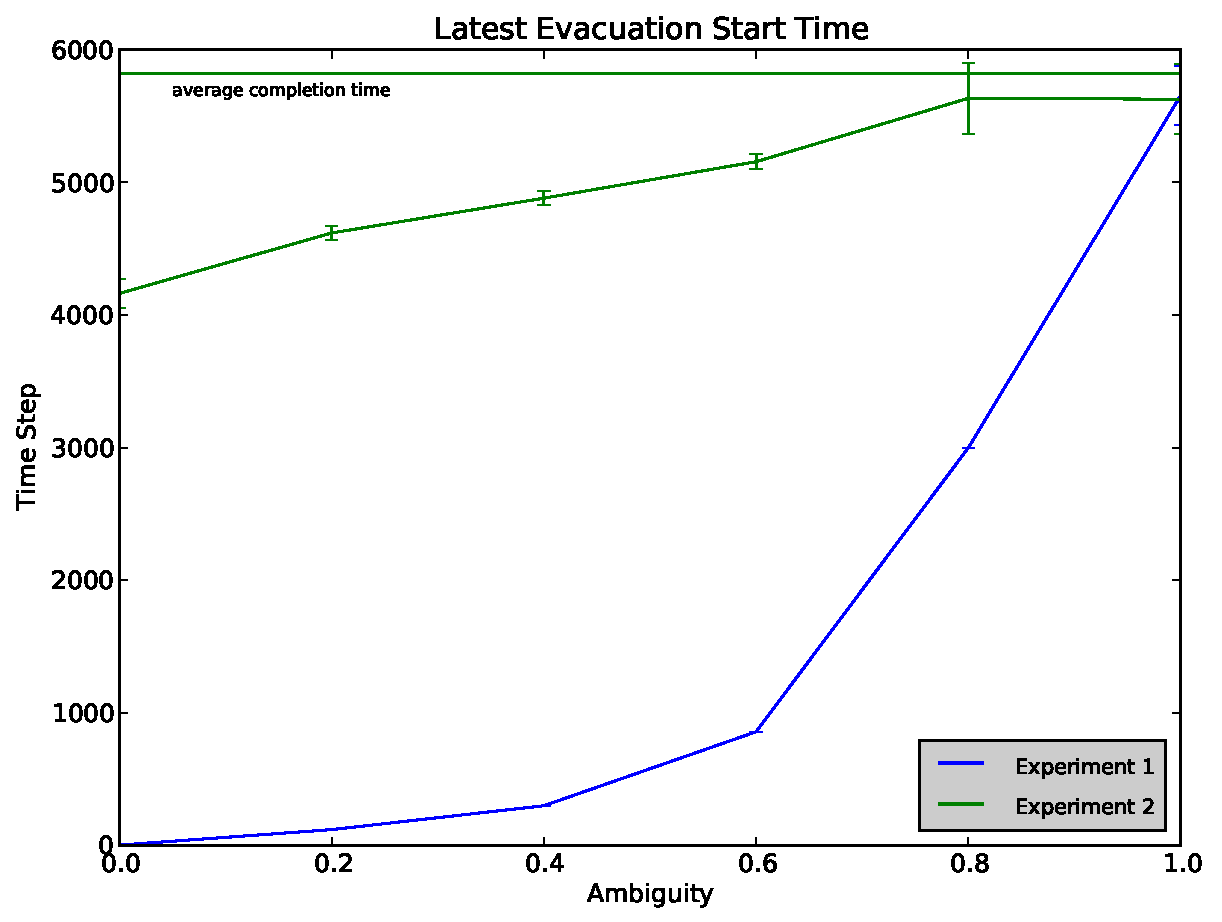
\includegraphics[width=6cm,height=6.2cm]{Exp2}}
  \caption{Observations from 100 replications of each setting of the IBEVAC Simulation}
  \label{Exp4}
 % Change graph to have average survival rate instead of average number survived.
\end{figure}


\section{Conclusion and Future Work}
\label{ConclusionAndFutureWork}

In this paper, the IBEVAC agent architecture for agent based simulation of emergency egress was introduced. A novel cue modeling and perception system which enables the detailed modeling of pre-evacuation behavior has been described and its working demonstrated.

Only preliminary experiments and results were presented in this paper. Further experiments are being conducted in examining the effect of partial knowledge, variability in trustworthiness and other factors. An interesting extension to the cue perception system would be the implementation of a cue memory. This can be used to model agents forgetting about certain cues or being desensitized to cues due to overexposure.